%%%%%%%%%%%%%%%%%%%%%%%%%%%%%%%%%%%%%%%%%%%%%%%%%%%
%
%  Author: Jacob Vaughn
%  
%  Last Updated: 3/8/2024
%
%%%%%%%%%%%%%%%%%%%%%%%%%%%%%%%%%%%%%%%%%%%%%%%%%%%

%%%%%%%%%%%%%%%%%%%%%%%%%%%%%%%%%%%%%%%%%%%%%%%%%%%%%%%%%%%%%%%%%%%%%%
%%                         INTRODUCTION
%%%%%%%%%%%%%%%%%%%%%%%%%%%%%%%%%%%%%%%%%%%%%%%%%%%%%%%%%%%%%%%%%%%%%


\pagestyle{plain} % No headers, just page numbers
\pagenumbering{arabic} % Arabic numerals
\setcounter{page}{1}


\chapter{INTRODUCTION \& LITERATURE REVIEW}

\section{Introduction}

In recent decades, the continual improvement in hypersonic aerodynamics has emphasized the need for advancements in wind tunnel ground testing capabilities \cite{leyva}. Conventional hypersonic wind tunnels rely on distinct fixed nozzle contours to accelerate the flow to the desired Mach number. This approach fixes the Mach number so it only provides a particular flow regime for experiments. Recognizing this, there is a clear need for a continuously variable Mach-number nozzle designed to overcome the limitations of conventional wind tunnels and enable more advanced dynamic hypersonic research.

The objective of this work is to introduce a continuously variable and actively controllable Mach-number nozzle. By dynamically adjusting the throat height and thereby the Mach number throughout the wind tunnel runs, the variable conditions experienced by hypersonic vehicles during different flight trajectories can be effectively modeled. This capability would enable the advancement of ground testing for a more comprehensive understanding of dynamic hypersonic flight and associated phenomena. Furthermore, the active control capability will increase experimental efficiency by allowing measurements at different Mach numbers within a single run and introduce the ability to fine tune the Mach number for improved data quality. However, this variable Mach number capability does introduce the challenge of maintaining desired Reynolds numbers, so feedback control will also be explored for the Reynolds number to counteract this and improve the overall experimental control.

The Actively Controlled Expansion (ACE) wind tunnel at Texas A\&M University has served as a workhorse in hypersonic research since 2010 \cite{ace09,ace10-calibrate,tichenor-dis,aceturb,mai-dis,neel-dis,leidy-dis}, and is due for improvements to meet the growing demand of hypersonics research. Although the facility was initially designed to facilitate the continuous variation of Mach number, the mechanical implementation ultimately proved to be cumbersome to adjust. Consequently, the nozzle has remained fixed at Mach 6 for the majority of the tunnel's operation, \textcolor{red}{falling short of fully realizing its designated variable Mach capability}. Additionally, despite the geometry being fixed, the Mach number actually varies throughout a run by up to 5\%. \textcolor{red}{Considering this, it is apparent that an update to the ACE nozzle is necessary to remedy these shortcomings.}

\section{Research Objectives}

The objectives of this research aim to lay the foundation for continuously variable and actively controlled Mach number capabilities at the National Aerothermochemistry and Hypersonics Laboratory (NAHL). Doing so will expand the current capabilities within the lab for more advanced hypersonic aerodynamics experiments. This will help maintain the NAHL as a cutting-edge national research facility. The existing ACE facility will be upgraded to achieve true active control and to potentially produce low-disturbance flow for higher Reynolds numbers. Its successor, ACE2.0, that is the subject of this work, will employ a feedback-control system with servo motors, linear actuators, and various instrumentation to enable the accurate and continuous variation of Mach number by changing the throat height. Additionally, active feedback-control of the Reynolds number will be developed and potentially implemented. 

Once fabricated and calibrated, the ACE2.0 facility will provide:

\begin{enumerate}[listparindent=\parindent]
    \item Improved experimental control and efficiency
            
        An active throat height control system will be implemented to enable active feedback-controlled Mach number variation and selection for Mach trajectories and accurate set points. The feedback aspect will attempt to control the Mach number to within 0.5\% of the set value. An active control scheme will also be developed to enable feedback-controlled Reynolds number variation and selection that responds to changes in Mach number and stagnation temperature for accurate sweeps and set points. This will allow both constant or varying Reynolds number during a Mach trajectory. The Reynolds number controller will be fully designed but may not be implemented due to constraints.

        The control of both of these parameters will yield improved experimental efficiency with a new capability to explore multiple flow configurations within a single run. Besides enhancing efficiency, the Mach number and Reynolds number control will enable more robust uncertainty quantification and more dynamic experiments that were not possible before. Both of these capabilities are demonstrated in the next objectives.

    \item Characterization of freestream flow uniformity and disturbance levels throughout the nozzle and uncertainty quantification of flow parameters

        A flow survey of the nozzle exit plane and centerline will be conducted to measure the freestream flow uniformity and disturbance levels throughout the nozzle and characterize its performance. This will validate the design and manufacturing of the nozzle and settling chamber and provide a basis for the quality of data gathered in future experiments. A rigorous uncertainty analysis will be performed to quantify the systematic and random uncertainty of the measured flow parameters $P$, $P_0$, and $T_0$ and the resulting values of Mach number, $M$, and unit Reynolds number, $Re'$. This will establish the baseline uncertainty for the freestream flow parameters and enable improved data quality for future experiments. In order to fully characterize the tunnel behavior while actively controlled, an investigation of the potential existence of hysteresis phenomena will be performed. If discovered, any hysteresis will be characterized to fully understand the dynamics of the freestream flow as each parameter is varied.

    \item Demonstration of Mach trajectory operation and potential hysteresis in a proof of concept experiment

        The capabilities of ACE2.0 will be demonstrated in an experiment that will showcase shock wave interactions between two wedges during a Mach trajectory. This experiment will explore a well-known hysteresis in the transition from a regular reflection to a mach reflection and the ability to produce the phenomenon in this facility. 

\end{enumerate}

These objectives will effectively validate and demonstrate the capabilities and merit of the new ACE2.0 facility. In addition, the standard operating procedures for ACE2.0 will be updated to reflect the best practices deduced throughout the completion of these objectives. The resulting control procedures and interface will be straightforward and well documented so that future users can easily learn to effectively operate the facility. The documentation will not only enhance the accessibility of ACE2.0 for subsequent research endeavors but also contribute to the broader scientific community by providing a robust framework for effective wind tunnel control and dynamic hypersonic vehicle aerodynamics exploration.

\section{Literature Review}

The literature review for this dissertation includes four parts related to hypersonic variable Mach-number wind tunnels and according to the above objectives: (1) variable mach number nozzle design, (2) parameter control, (3) flow quality characterization and uncertainty quantification, and (4) hysteresis in hypersonic flows. This review will discuss articles that establish the most current knowledge base and techniques in the relevant areas of hypersonic wind tunnel research.

\subsection{Variable Mach-Number Wind Tunnels}
Variable Mach number nozzles have been explored in many configurations since the 1950s such as interchangeable fixed-block, plug-type, asymmetric sliding blocks, tilting plate, fully flexible, and hinged/flexure \cite{agard-ag-3}. Each of these designs have varying degrees of flow quality, cost effectiveness, and experimental efficiency that must be considered. Only the fully flexible and flexure designs maximize experimental efficiency without sacrificing flow quality. Of these two, the flexure design minimizes costs by reducing mechanical complexity and supporting structure. Therefore, the flexure design is the optimal choice considering these criteria.

The flexure type nozzle was first proposed in 1955 by Rosen \cite{rosen} and improved upon separately by Erdmann in 1971\cite{erdmann} and Rom and Etsion in 1972 \cite{erdmann,rom} in order to minimize the mechanical complexity. This simple nozzle design operated by a single jack greatly reduces manufacturing and controls costs and allows for greater flexibility in active control to quickly and continuously vary the Mach number to model dynamic supersonic vehicle flight.

In the last decade, many variable mach number supersonic wind tunnels have been manufactured due to increased demand of hypersonic flight research. The majority of these are fully flexible or flexure nozzle designs with varying implementations of actuation and control \cite{ilic-1,shahrbabaki-1,durand,laguarda,chen,guo,lv,qi,steeves}. All of these facilities were developed to study vehicle flight trajectory and the hysteresis phenomenon therein.

\textcolor{red}{Duplicate at start of chapter 2?} The ACE tunnel, the facility of interest for this work, has been in operation since 2010 \cite{ace09,ace10-calibrate,tichenor-dis}. The nozzle is a flexure type that produces Mach 5 to 8 flow in a 9 inch by 14 inch test section. The flexure design is effective in achieving the change in throat height, but it cannot be done continuously and actively during a run. This is the primary issue to be addressed in this work.

\begin{figure}[ht!]
    \centering
    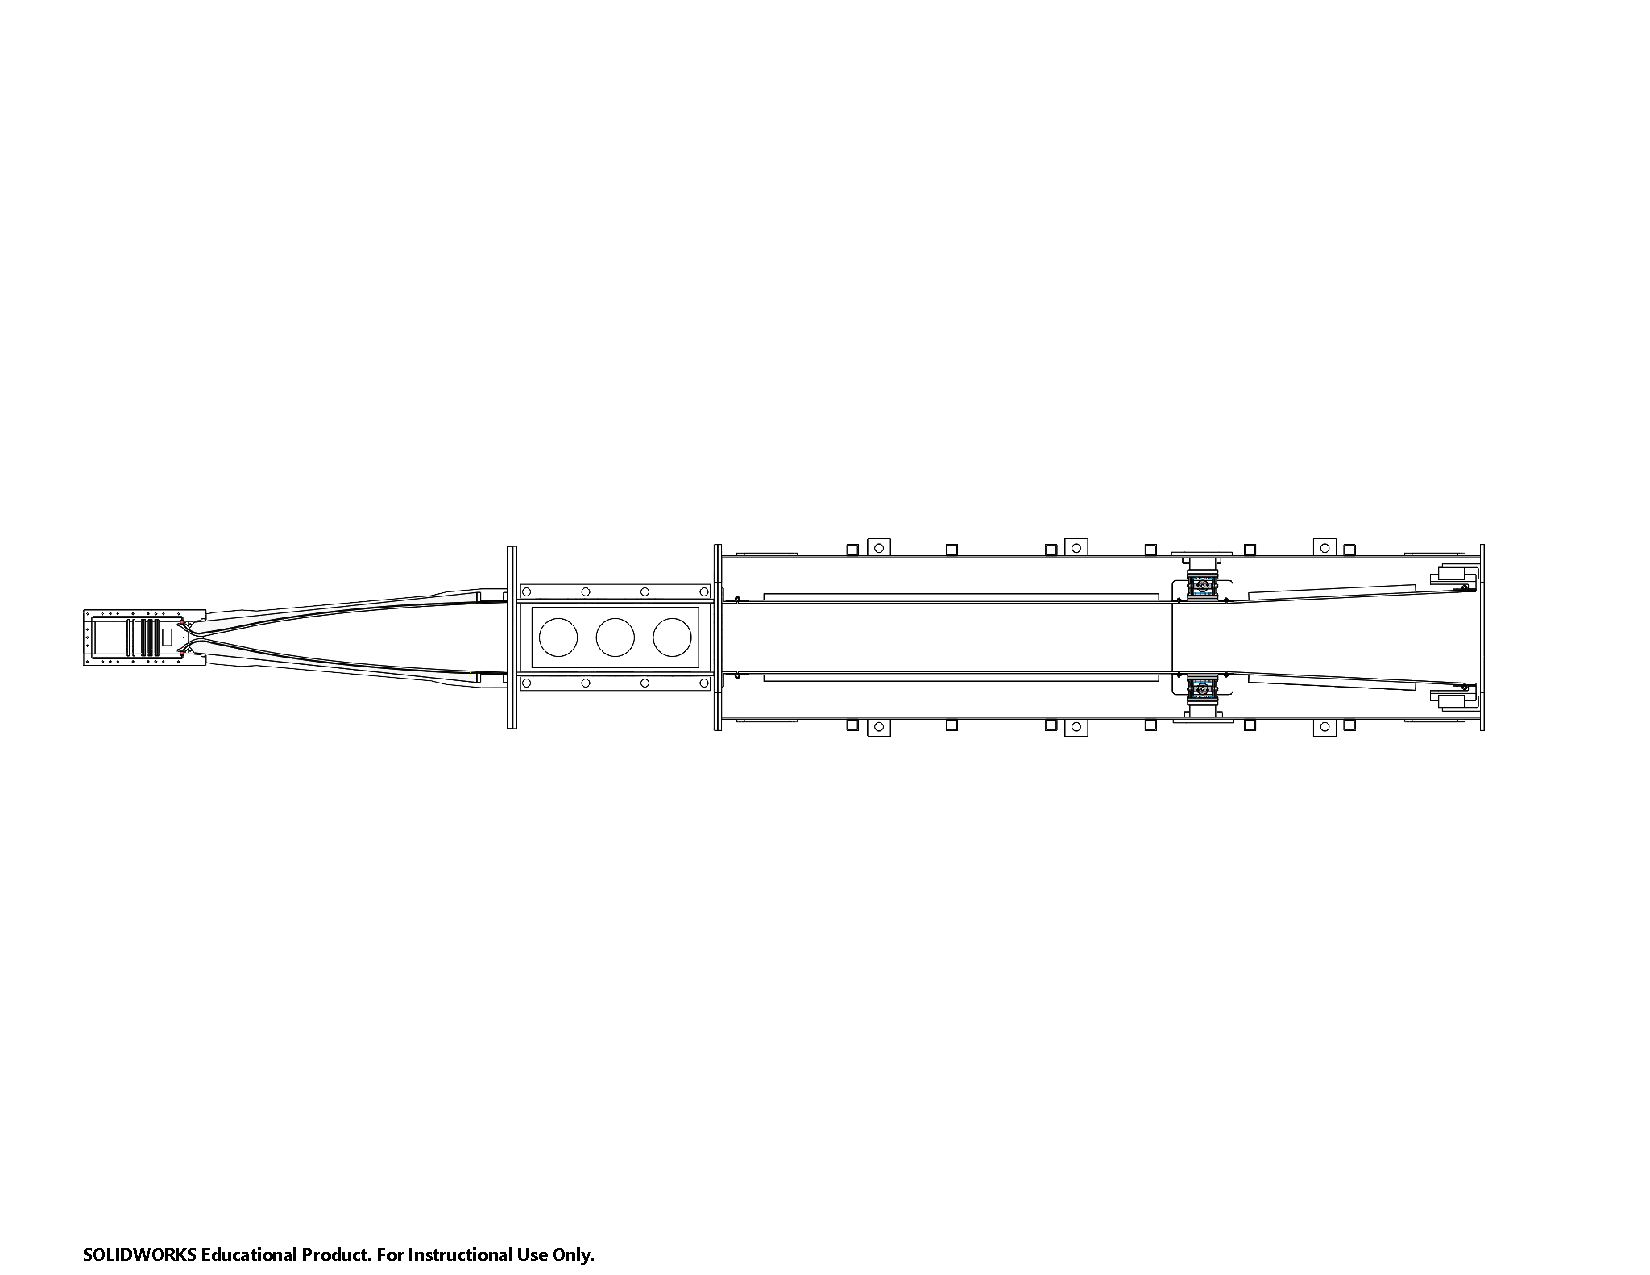
\includegraphics[trim={40 250 60 250},clip,width=6in]{ace-full-tunnel.pdf}
    \caption{ACE tunnel schematic}
    \label{fig:ace-full-tunnel}
\end{figure}

\subsection{Parameter Control}
A variable Mach number facility requires effective control schemes for the controllable parameters $A^*$, $P_0$, $T_0$, and the resulting Mach number, $M$, and unit Reynolds number, $Re'$, in order to vary each parameter independently and accurately. This control problem, acknowledged as early as the 1980s, prompted the development of diverse solutions implementing the various areas of control theory such as optimal control \cite{kraft,hwang}, state feedback control, mathematical model prediction control, preprogrammed controllers \cite{matsumoto}, and PID control \cite{fung,ilic-2,silva}.

In recent years, researchers at numerous variable Mach number facilities have embraced advanced intelligent control methods. Techniques such as fuzzy logic, genetic algorithms, neural networks, adaptive control or gain scheduling, and their combinations have been applied \cite{nott,shahrbabaki-1}. The methods that will be explored in this research are those of Hwang et al. \cite{hwang}, Matsumoto et al. \cite{matsumoto}, Ili\'c et al. \cite{ilic-2}, and Shahrbabaki et al. \cite{shahrbabaki-1} as they each introduce the different advantages and challenges of each control technique. 

Hwang et al. \cite{hwang} developed a robust LQG/LTR (Linear Quadratic Gaussian with Loop Transfer Recovery) controller enhanced by an anti-integrator windup and a modified Smith predictor to overcome unavoidable modeling errors, uncertainties, and time-delay effects. This controller demonstrated a faster stabilization and exhibited fewer oscillations in comparison to its PID counterpart. Given its superior performance, it presents an appealing prospect for implementation in ACE2.0, and a detailed exploration of this controller will be undertaken in a subsequent chapter.

Matsumoto et al. \cite{matsumoto} took a simplified approach by replacing an existing real-time PID controller with a preprogrammed controller to avoid input time delays. This was advantageous for the facility used in that work because the run time was not much longer than the time delay for the PID controller to stabilize. This is the most straightforward approach to obtain specific constant or dynamic trajectories of multiple input parameters but it has limitations. The controller must have a new program for each individual desired parameter set condition or path, and each program must be iterated to minimize errors. Considering these limitations, a preprogrammed controller will be a backup option that will only be explored if necessary. Considering the longer run times of ACE2.0, a PID controller can be implemented with ample time to stabilize.

Ili\'c et al. \cite{ilic-2} implemented a cascade nonlinear feedforward-feedback PID controller as a combined system to enhance a standard single-loop PID. The system's set point reference tracking is improved by the feedforward-feedback architecture, and the disturbance rejection is improved by the cascade architecture. With these two architectures combined in one multi-loop controller, large transient overshoots are eliminated, set point settling times are decreased, and the overall accuracy of the controlled parameters is maximized. Once again, the improved performance of this controller makes it another appealing prospect for ACE2.0, which will be discussed later.

Shahrbabaki et al. \cite{shahrbabaki-1} utilized an artificial neural network and fuzzy logic to enhance a conventional PD controller to handle the complex nonlinearity of the variable mach number wind tunnel flow parameters. The advantages of fuzzy logic include its simplicity and adaptability of introducing new control rules to handle imprecise data, uncertainty, and unmodeled dynamics. The combined advantage that Shahrbabaki et al. explores pertains to the utilization of the neural network to develop the membership functions for the fuzzy logic controller. They designed and trained a feed-forward multilayer perceptron neural network according to the database from the mathematical model of the wind tunnel behavior in order to develop the optimal membership functions. This method will only be explored further for ACE2.0 if the methods of Hwang et al. or Ili\'c et al. do not yield sufficient performance.

\subsection{Flow Quality Characterization and Uncertainty Quantification}
The primary references regarding flow quality characterization will be the recent AIAA articles by Chou et al. \cite{chou} and Duan et al. \cite{duan} on hypersonic wind tunnel freestream disturbance measurements. These provide the latest measurement processes and procedures and reference over 50 publications on relevant topics from recent decades. In addition to these two references, a decade of NAHL experience and best practices will guide the characterization of ACE2.0 upon its fabrication and initial shakedown. Key NAHL ACE references on the freestream characterization of ACE are the AIAA paper by Semper et al. \cite{aceturb} and multiple dissertations by Mai \cite{mai-dis}, Neel \cite{neel-dis}, and Leidy \cite{leidy-dis}. Additionally, Leidy performed an uncertainty analysis in the existing ACE tunnel that will provide a rough baseline reference for the uncertainty quantification for ACE2.0.

The primary references for the uncertainty quantification in this research will be the NASA report by Stephens et al. \cite{stephens-hubbard}, the forthcoming AIAA Guide on Uncertainty Quantification \cite{uq-aiaa}, and the dissertation by Curriston \cite{curriston-dis}. The methodology in this NASA report combines the techniques of the prevalent literature on the subject from the last few decades to quantify the uncertainty of the flow parameters in a supersonic wind tunnel. Curriston's work provides a secondary reference as he thoroughly demonstrates this methodology and that of the forthcoming AIAA guide as a case study in a low speed wind tunnel. The approach described in these references includes a sophisticated treatment of systematic uncertainty using a Mont Carlo method combined with direct comparison of replicate data to characterize random error. Curriston \cite{curriston-dis} also extensively treats pre-test and real-time uncertainly quantification to enhance test campaign quality control and decision support.

\subsection{Hysteresis in Hypersonic Flows}
A review of the literature on hypersonic flow hysteresis yielded many publications discussing shock interactions and inlet start/unstart processes. The inlet start/unstart literature will not be referenced directly in this work but will be valuable for future research in ACE2.0. Focusing on the shock interactions, Hornung et al. \cite{hornung-1} first predicted hysteresis in the transition from regular reflection to Mach reflection, but they were unable to experimentally produce the hysteresis effect \cite{hornung-2}. Recent literature reveals numerical investigations easily reproduce shock interaction hysteresis \cite{chpoun-1,ivanov-3}, while experimental investigations prove more difficult due to the freestream noise in conventional facilities \cite{ben-dor-1,laguarda}. The two processes that produce hysteresis in the shock interactions are wedge-angle variation and Mach-number variation \cite{ben-dor-2}. Since it is significantly more complex to vary the Mach number, most experimental results are found by the wedge-angle-variation-induced hysteresis in open-jet, low-noise wind tunnels \cite{chpoun-2,li,ivanov-4,mouton,setoguchi,chanetz}. Some research groups with variable Mach number tunnels have attempted to reproduce shock interaction hysteresis experimentally by varying the Mach number, but they have all been unsuccessful due to the presence of high freestream disturbance levels \cite{durand,tao}. Methodologies from the numerical and experimental literature on Mach-number-variation-induced hysteresis will be studied in order to attempt to reproduce shock interaction hysteresis in ACE2.0.

